\section{Algorithm Distillation on Permuted Train Sets}
\label{appendix:ad_perm}

\begin{figure}[h]
    \vskip 0.2in
    \centering
    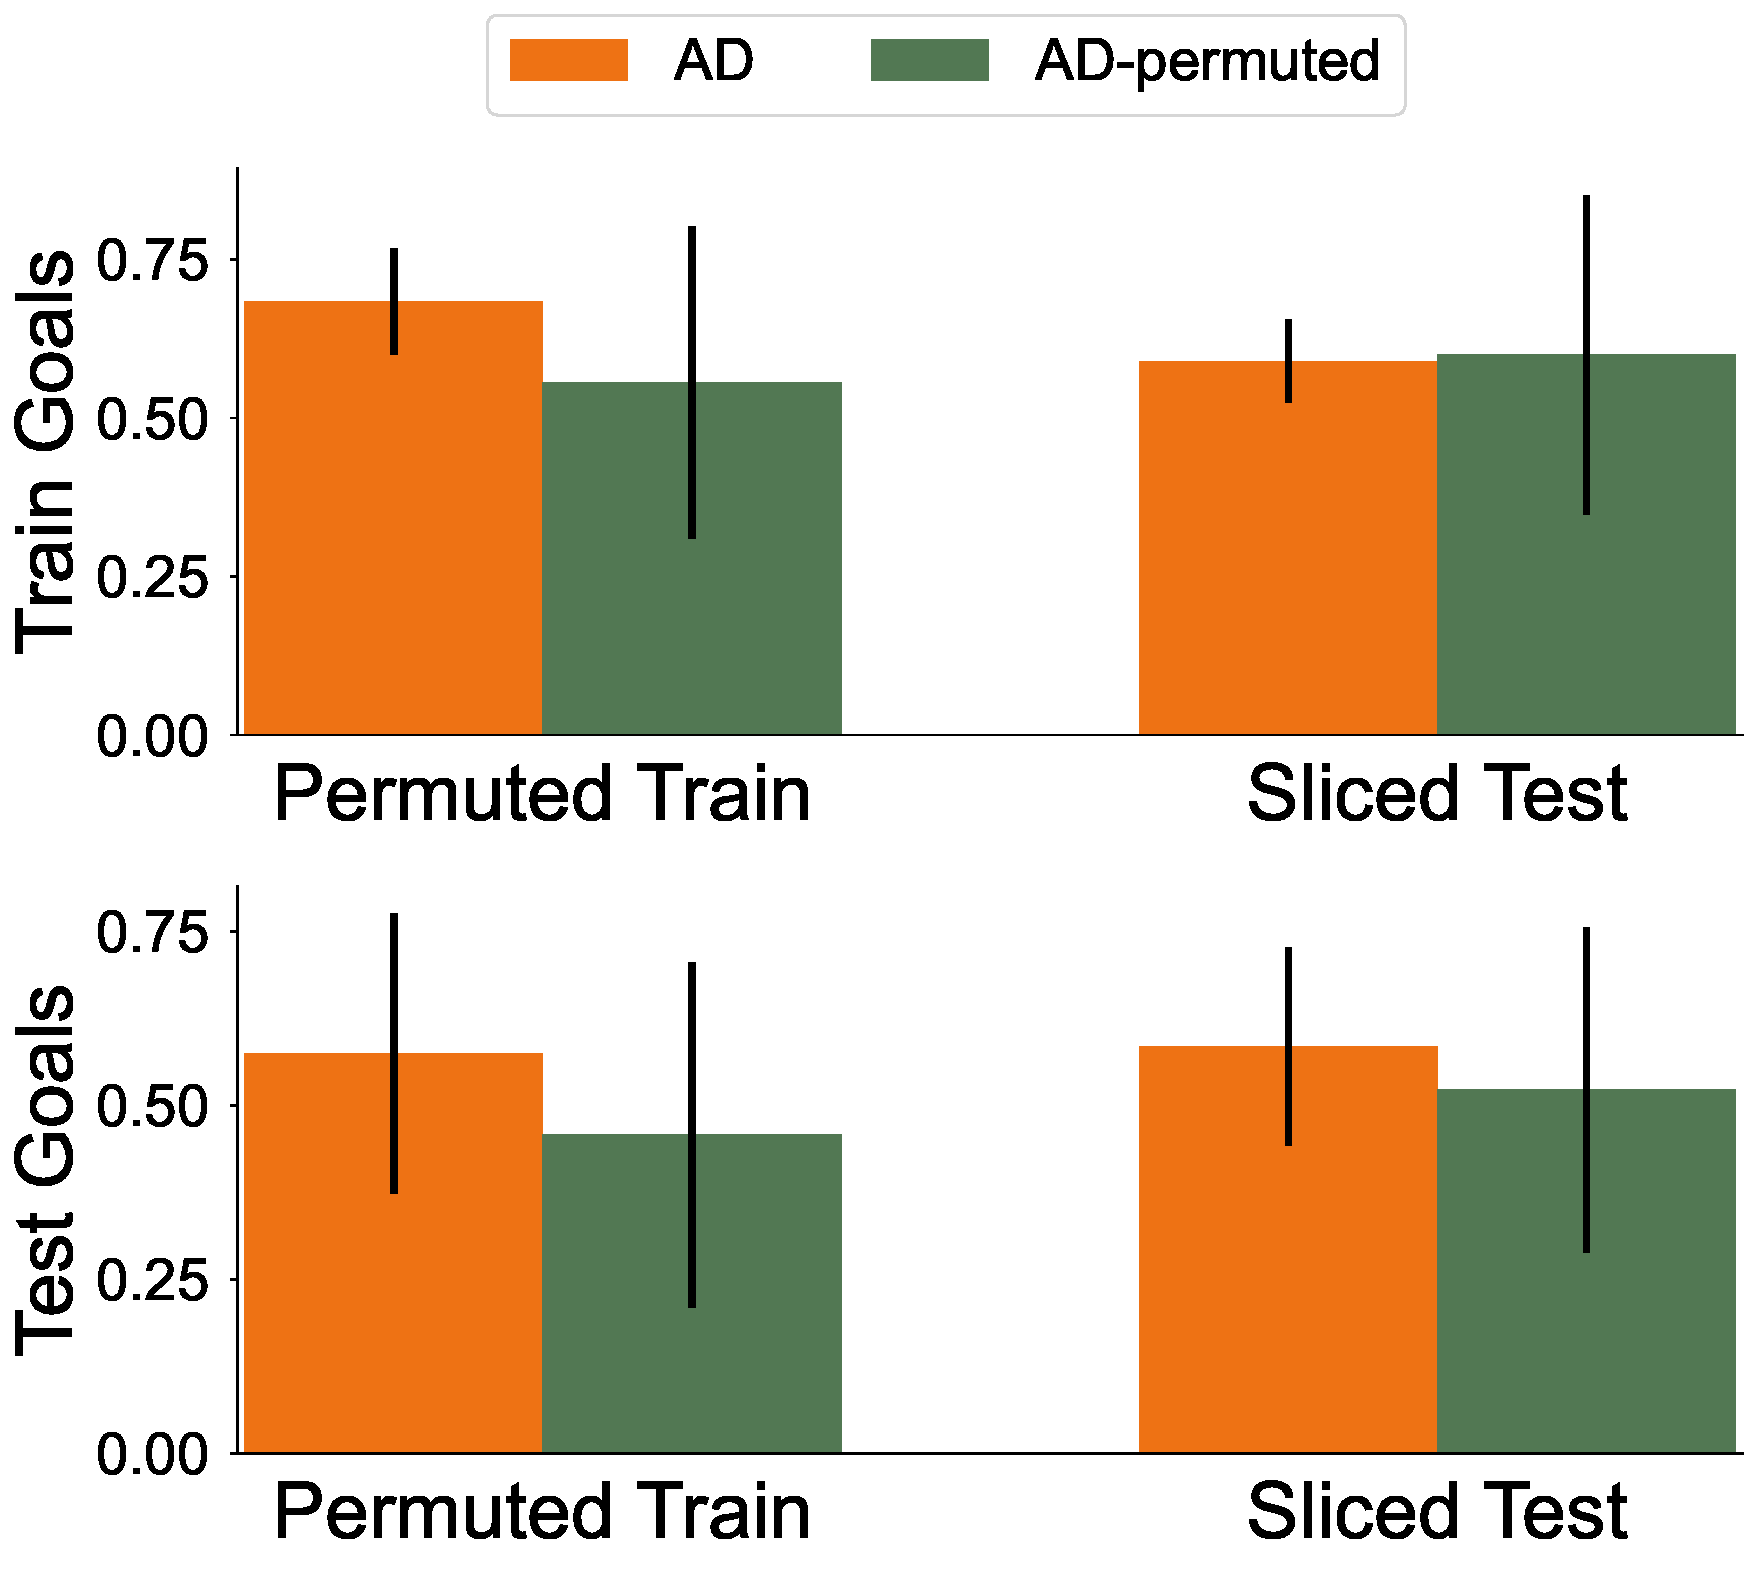
\includegraphics[width=0.35\columnwidth]{images/gridworld_vanilla_perm.pdf}
    \caption{\textbf{AD Performance on Permuted Actions:} This figure shows the models' success rates on Darkroom environment, averaged over $5$ seeds. We evaluated AD's ability to adapt to action sets with varied semantics by training it on a permuted dataset. Except for this, the training and testing are the same as in the vanilla setting and can be found in \Cref{sec:exp_gridworld}. Contrary to expectations, this tailored training did not enhance performance when compared to the AD model trained on standard datasets.}
    \label{fig:gridworld_vanilla_perm}
    \vskip -0.2in
\end{figure}